%
%  normalEstimators
%
%  Created by Daniel Beatty on 2007-10-19.
%  Copyright (c) 2007 Texas Tech University. All rights reserved.
%
\documentclass[11pt]{article}
\usepackage{geometry}                % See geometry.pdf to learn the layout options. There are lots.
\geometry{letterpaper}                   % ... or a4paper or a5paper or ... 
%\geometry{landscape}                % Activate for for rotated page geometry
%\usepackage[parfill]{parskip}    % Activate to begin paragraphs with an empty line rather than an indent
\usepackage{../../doublespace}
\usepackage{../../algorithm,../../algorithmic}
\usepackage{graphicx}
\usepackage{amssymb}
\usepackage{epstopdf}
\usepackage{listings}

%\usepackage{algorithm,algorithmic}
\DeclareGraphicsRule{.tif}{png}{.png}{`convert #1 `dirname #1`/`basename #1 .tif`.png}

\newtheorem{thm}{Theorem}[section]
\newtheorem{adef}[thm]{Definition}
\newtheorem{cor}[thm]{Corollary}
\newtheorem{lem}[thm]{Lemma}


\title{Introducing Neighborhood Algebra with Another Solution for Principal Component Analysis}
\author{Dan Beatty}

\begin{document}
\maketitle

\section{Introduction}
Concepts of Principal Component Analysis (PCA) have now been used in mathematical, scientific, and engineering applications for longer than a quarter century, at the time this paper was written.   It is a process of acquiring an estimation mixing matrix, and applying that matrix to map a given data set to an orthonormal basis.  In some definitions, the properties of zero mean and unit covariance are essential to the process.  In other cases, those properties are more liberally interpreted.  Computationally, the methods for determining PCA have become classic and up until the most efficient ways relied on convergence to limit the number of computations required to find the estimate.   Section \ref{math-overview-section} provides a formal review and comparison of the two classic methods of satisfying PCA, both Eigenvalue Decomposition (EVD) and Gram Schmidt Orthogonalization (GSO.)   %The mathematics of PCA are shown in detail in section \ref{-overview-section}.

Another trend in computing hardware emerged that challenges these conventional methods of computation.  These trends are for specialized hardware to be included with general purpose hardware to provide the augmented capabilities of both.   Graphics cards are a commonly available form of hardware trend in this trend.  %One of these specialized configurations is conveniently available on most present day machines, namely the graphics card (and the processor on that machine.)  
The processors on these cards are efficient at floating point vector computations.  Typically, the processors on these graphics cards are commonly called graphics processing unit(s) (GPU(s)) and that nominclature is used in this paper as well.   %The constraints on these processors for new mathematical algebra and models to guarantee results and performance.  
GPUs constrain the use of branch oriented structures such as loop and conditional to either compile time or single instruction no-branch instructions.  This constraint is responsible for the speed and efficency of GPU.  The same constraint also challenges algorithms typically designed for generic central processing unit(s) (CPU(s).)   Section \ref{compuational-motivation} reviews the classical computing using these CPUs since Alan Turing's and Alonzo Church's thesis,  and explains the motivation of redesigning algorithms for GPU augmented architectures.    Algorithm designs intended to run on the GPU are commonly called GPU bound, and this paper obeys this convention.  
%These graphics processors have some constraints, which are responsible for the graphics card's success and speed.  
%The same constraints also require a mathematics (algebras) that respect these features.
GPU bound design motivates the need for an algebra that ensures successful GPU bound algorithms.  

This paper introduces one such algebra and applies that model to the classic concept of PCA.  %In the process, 
This new extension to linear algebra called Neighborhood Algebra (NA) takes one of the more deterministic forms of PCA to produce programs that run on the graphics card, which removes the need for convergence testing.  The properties of the NA operations reduce the need for substantial branching.   %It is this algebra that addresses on of the fundamental constraints of the graphics cards and other vector processors, namely the ability to restrict branching to allow for longer pipelines and shorter computation times. 
Neighborhood algebra itself is defined in section \ref{neighborhood-algebra}.  

%The mathematical overview presented in section reviews PCA in terms of both EVD and GSO.  These are provided so that the reader may have an understanding both means of satisfying PCA.   Another section is provided show the motivation of this algebra and this paper defining that algebra.  The last sections demonstrate the methods of implementation and the results 

%This paper presents this exploration in a number of sections.  The second section presents the mathematical background for PCA, and credits the initial researchers who introduced the world to these concepts.  The third section credits the modern history of computation, the constraints imposed by what is considered by this paper as conventional computation.  The fourth section introduces the concepts of NA.   In the fifth section, implementation of a prototype for NA is discussed.   In section six, the results of the implementation described in section is presented.   % One thing reserved is the model for operation objects to accelerate the building of these graphics card based programs.   




\section{Mathematical Overview of Principal Components}\label{math-overview-section}

%Expected Maximization (EM), Linear Discriminant Analysis (LDA), and Principal Component Analysis (PCA) can each be classified as a family of estimators.  Classically known estimators %classically known  include  least squares and maximum likelihood, which differ by their method of convergence.  LDA is a special case of Multiple Discriminant Analysis  (MDA) where the number of discriminants is reduced to two.

PCA falls in a family of classification techniques called estimators.  An estimator is a procedure that finds parameters of a model that closely fits a given data set.  PCA estimates the mixing matrix (also called transformation matrix in some texts) for a given set of data.   The PCA estimator (family of estimators) satisfy the PCA characteristic equation (equation \ref{pca-characteristic}) with least amount of error.  PCA restricts this error determination to the scatter matrix of a data set, typically called a background scatter matrix. 

A background scatter matrix is the scatter matrix for the entire collection of data points.  In practice, it is more useful to determine a scatter matrix for a reasonable sampling of the data than to use the entire data set.   %From such a background scatter matrix, the principal components can be determined.
%This background scatter matrix is useful in determining principal components.   
Principal components were defined by Moon and Stirling in the following way:

%\subsection{Principal Components}\label{pca-sub-section}

\begin{quote}
	The principal components of the observed data are selected so that the ith principal component is the linear combination of the observed data that accounts for the ith largest portion of the variance in the observations.
\cite[329]{moon-stirling-book}
\end{quote}

Let $\vec{x}$ be a sample from the observed data whose space is denoted $\mathbf{X}$.  Let $\vec{y}$ be the principal components of $\vec{x}$.  Then there is a transformation matrix $\mathbf{P}$ such that %equation \ref{pca-characteristic} is satisfied.
\begin{equation}
\vec{y} = \mathbf{P}\vec{x} \label{pca-characteristic}
\end{equation}
In order for $\mathbf{P}$ to satisfy equation \ref{pca-characteristic},  it should maximize equation \ref{pca-optimization-definition}, where $J(\cdot)$ is a least squared error minimization  function.  One nice characteristic for equation \ref{pca-optimization-definition} to have is that each vector in $\mathbf{P}$ be shown in equation \ref{pca-optimization-derivation} and \ref{pca-optimization-constraint}.  These constraints are satisfied by the eigenvectors of the scatter matrix of the selected $\vec{x}$.  
\begin{equation}
J(\mathbf{P}) = E\{ \vec{y}^2 \}  \label{pca-optimization-definition}
\end{equation}
%Most texts show that for each column vector of $\mathbf{P}$ to have a derivation as shown in equation \ref{pca-optimization-derivation}.  The important feature of $\mathbf{P}$ to be noted is that the eigenvectors of the covariance matrix of $\mathbf{X}$ are ordered by matching eigenvalues. 
\begin{eqnarray}
J(\vec{p}_1) = E \{ y^2 _1 \} = E \{ (\vec{p}_1^T \vec{x} )^2 \} = \vec{p}_1 ^T E \{ \vec{x}\vec{x}^T \} \vec{p}_1 \label{pca-optimization-derivation} \\
 || \vec{p}_1 || = 1 \label{pca-optimization-constraint}
\end{eqnarray}
%Note that any 
Any $\mathbf{P}$ that satisfies the constraints of PCA is a valid PCA transformation matrix.  
Singular Value Decomposition, Karhunen-Loeve,  Hotelling transforms, Givens, and Pearson all acquire the transformation matrix that determines the principal components.  %The constraint on $\vec{x}$ being of zero mean and unit covariance can be relaxed, so long as $\mathbf{P}$ is still kept orthonormal.
The eigenvalues and eigenvectors of the data's scatter matrix comprise one form of principal components.  The resulting matrix formed from these eigenvectors produce a the principal component mixing matrix shown in equation \ref{data-by-principal-component}.
In this case, there is an assumption that each data vector $\vec{x}$ is defined in terms of some mixing matrix, $\mathbf{P}$, a matching set of principal components $\vec{a}$, and a mean vector $\vec{\mu}$.   The mean can for practical purposes be the sample mean of $\vec{x}$.  
Equation \ref{principal-component} shows the inverse relation of principal component to data vector.  Also, the zero mean requirement can be relaxed in some cases.
\begin{eqnarray}
\vec{x} = \vec{\mu} + \mathbf{P}\vec{a} \label{data-by-principal-component} \\
\mathbf{P}^T(\vec{x} -\vec{\mu}) = \vec{a} \label{principal-component} \\
\vec{x} = \vec{\mu} + \sum _i a_i \vec{e_i} \label{data-by-principal-component-eigenvector} 
\end{eqnarray}

%For CPU bound computation of PCA, SVD is a classic well known algorithm that is part of the LAPACK libraries and has  acceleration via the Accelerate framework \cite{apple-accelerate-framework}.  Also, the LAPACK implementation for EVD is also prudent for determining principal components when computation is CPU bound. For GPU bound, both classic methods and online methods should be considered. In process of considering these methods, the cost metrics for GPU bound computation is significantly different than classic CPU bound computation due to the constraints of computation.


The following two subsection describe both Eigenvector Decomposition (EVD) and Gram-Schmidt Orthogonalization (GSO), which was named after Jorgen Gram and Erhard Schmidt (1907).  Both procedures are well known methods for obtaining an orthogonal matrix, which will satisfy the mixing matrix.  %EVD is included in LAPACK, and already has a CPU bound implementation which has been optimized via the Accelerate Framework.  GSO is a better candidate for GPU bound computations as it can be constructed via modules that are zero-branch, and the number of those modules is function of size, not convergence.  


\subsection{Gram-Schmidt Orthogonalization}
PCA requires the transformation matrix to orthonormal, and this is typically satisfied by EVD. %are defined by a transformation matrix which is orthonormal and typically consisting of eigenvectors. 
Therefore any procedure that obtains an orthonormal matrix linearly equivalent to the scatter matrix constitutes a PCA method.  
One other estimate satisfying the requirement for such an orthogonal matrix is called Gram Schimidt Orthogonalization (GSO).    
Theorem \ref{gso-theorem} states that a vector space $\mathbf{V}$ can be transformed into another vector space $\mathbf{W}$ such that each $\vec{w}\in \mathbf{W}$ is orthogonal.  GSO is a procedure based on theorem \ref{gso-theorem} that constructs each $\vec{w}_i \in \mathbf{W}$ one right after the other, and is defined in algorithm \ref{alg:gso}. 

\begin{quote}
\begin{thm} 
\label{gso-theorem}
Suppose $w_1, w_2, ..., w_n$ form an orthogonal set of non-zero vector in $\mathbf{V}$.  Let $v$ be any vector s.t. $v \in \mathbf{V}$.  Define $v'$ s.t. 
\begin{eqnarray}
v' = v - c_1 w_1 - c_2 w_2 - ... - c_n w_n \label{GSTheorem}\\
c_i = \frac{\langle v , w_i \rangle} {||w_i||^2}
\end{eqnarray}
Then $v'$ is orthogonal to $w_1, w_2, ..., w_n$.
\end{thm} \cite[211]{schaums-linear-algebra}
\end{quote}


\begin{algorithm}
\caption{Gram Schmidt Orthogonalization}
\label{alg:gso}
\begin{algorithmic}
	\REQUIRE Column Wise Source Matrix: $\mathcal{V}$
	\STATE $N$ is the number of column vectors in $\mathcal{V}$
	\STATE Base case $\vec{v}_0 = \vec{w}_0$ 
	\STATE initialize $\vec{\theta}^0$, $T$, and $i \leftarrow 0$
	\STATE $v_0 \leftarrow $ [V columnVector:1]
	\STATE [W insertVector:$v_0$ atColumn:1]
	\FOR {j = 2 to N}
		\STATE $v_j \leftarrow$ [V columnVector:j]
		\FOR {i = 1 to j}
			\STATE $(w_i)_{\textsl{norm}} \leftarrow ||w_i ||$  
			\STATE innerProduct ($i_p$)$\leftarrow$ $\langle w_i , v_j \rangle$
			\STATE \textsl{negsum} += $i_p / (w_i)_{\textsl{norm}}$
		\ENDFOR
		\STATE result = $v_j - \textsl{negsum}$
		\STATE [W insertVector:result atColumn:j]
	\ENDFOR
%	\RETURN 
	\ENSURE $W$
\end{algorithmic}
\end{algorithm}

\subsection{Eigenvalues: Characteristic Polynomials}
\begin{quote}
	\begin{adef}
		Consider an $n$-squared matrix $\mathbf{A}$ over a field $\mathcal{K}$
		\begin{equation}
			\mathbf{A} = 
			\left(
			\begin{array}{cccc}
				a_{11}  &a_{12}  & ... &a_{1n}     \\
				a_{21}  &a_{22}  & ... &a_{2n}     \\
				...& ...& ...&... \\
				a_{n1}  &a_{n2}  & ... &a_{nn}     \\
			\end{array}
			\right)
		\end{equation}
		The matrix $t\mathbf{I}_n - \mathbf{A}$ where $\mathbf{I}_n$ is the $n$-square identity matrix and $t$ is an intermediate, is called characteristic matrix of $\mathbf{A}$
	\end{adef}
	\cite[281]{schaums-linear-algebra}
\end{quote}
The determinant of the characteristic matrix is the characteristic equation (polynomial) of $\mathbf{A}$.  The definition for eigenvalues and eigenvectors is stated in the quoted definition \ref{eigenvalueDefinition}.
\begin{quote}
\begin{adef}
	\label{eigenvalueDefinition}
Let $\mathbf{A}$ be an $n$-square matrix over a field $\mathcal{K}$.  A scalar $\lambda \in K$ is called an eigenvalue of $\mathbf{A}$ if there exists a nonzero (column) vector $\vec{v}\in \mathcal{K}^n$ for which equation \ref{eigenvalueCharacteristicEquation} holds.
\begin{equation}
\mathbf{A}\vec{v} = \lambda \vec{v}  \label{eigenvalueCharacteristicEquation}
\end{equation}
Every vector satisfying this relation is then called an eigenvector of $\mathbf{A}$ belonging to the eigenvalue $\lambda$.
\end{adef}
\cite[284]{schaums-linear-algebra}
\end{quote}
There is a family of algorithms called Eigenvalue Decomposition (EVD) that finds the eigenvalues and eigenvectors.   EVD is part of the Linear Algebra Package (LAPACK) libraries and consequently part of the Accelerate framework\cite{apple-accelerate-framework}.  Thus for CPU bound operations, the LAPACK version is the best choice, as it is already optimized for the CPU.   



\section{History of Turing Models and difference between general and graphics processors}\label{compuational-motivation}
In this section, a brief review of classical computation on general purpose processor is presented.  Since the architecture for the general purpose processors place the processor as central to all operation of the machine, it has classically been called the central processor.  Also in this section, the trade off between pipelines and branches is presented, which shows where acceleration was introduced to CPUs and the constraints that limit each.   Lastly, graphics processors are introduced, which do not have the same constraints as a general processor. This distinction is shown with a path to exploit that difference.


% Differences come together
General and graphics processors can complement each other in addressing the branching and pipeline trade offs.  Graphics processors handle pipelines extremely well, but branches very poorly.  General processors handle branches well, and construction of their pipelines are constrained to accommodate such branches.  To achieve the best of both worlds, a hybrid approach should use one to augment the other so both processes accomplish tasks that they are optimized for.  



% Application toward graphics and image processing
%The graphics and games community has used pipeline accelerated hardware as early as the 90's.  These pipelines have provided a responsive environment for applications presenting otherwise complex material.  Improvements in these processors have been viewed mostly by the gaming and simulation communities in the level of detail that could be presented.   The one thing these processors compute extremely well are floating point numerical values between zero and one, and geometric structures.  


\subsection{Dawn of Acceleration}
Alan Turing \cite{turing-computable-numbers} introduced to the world a model of computing with provable design.  Lambda calculus, introduced by Alzono Church \cite{church-unsolvable-problems, church-logic-foundation-postulates} and Stephen C. Kleene\cite{kleene-lambda},  provided a mathematics to prove the outcome of a given computation model.  From these two, computation science was formally born with the methods to design structures that will compute all that is computable, and prove that it is.  

% Development of acceleration
During the same decades that Alan Turing and Alzono church were introducing the mathematics that define computations, scientists such as John von Neumann introduced refined architectures for achieving computation guaranteed by the Turing-Church thesis.   The field of computer architecture derived from von Neumann architecture and other architectures satisfying the Turing Church thesis are vast.   Hennessy and Patterson \cite{hennsessyPatterson} illustrated branch and pipeline as a classic tradeoff in processor design.  % a basic theme is the branch and pipeline.  


The concept of the pipeline is well known in the computer science community.  Each operation consists of micro-instructions, %Break operations down a basic set of operations
which can be executed simultaneously.  These micro-instruction are assembled so that operations linear enter % Assemble these operations 
%in a line such that each operation enters 
the processor parts of it are determined in stages.  %The conceptual place where these operations executed are called stages.  Once an operation enters a stage, the process for that stage executes.  Many stages are required to perform an operation completely.  As an operation leaves a stage, another enters.  Typically, each stage is made to execute at the same rate.  
The intended result of such the pipeline structure is that one whole operation is executed per cycle, after the pipeline is full.  %The constraint for all pipeline structures is the branch instruction.


\subsection{What are the general classical models?}
Classical models of computing PCA hinge on the von Neumann Architecture for processor design.  This particular architecture includes an arithmetic unit, a control unit, memory channels or blocks, and input/ output channels.   Since its conception in the 1940's, John von Neumann's architecture has been used to define methodologies of computation and processors to perform the computing.   It is this architecture where the term CPU bound is given its meaning.

% Introduction of the SISD architecture.
A special form of the von Neumann architecture was introduced by \cite{flynn-m-j} called single instruction single data (SISD).  The principle of SISD, as the name implies, is to execute on instruction with a single set of data per unit of execution.  %Once executed the 
The state of machine reflects the execution of previous instructions.  %The execution of any instruction is on the state of the machine at the time.  

%One of the caveats of the von Neumann architecture is that is a generalized design.  Many include pipeline structures to enhance their performance.   The constraint that these processors must obey is how to handle branches.  The volumes of work to optimize the trade off between the cost of branching versus pipeline speed is enormous.    
Classic computing models are based on three assumptions introduced by SISD architectures.  While these assumptions are true, %then
the iterative algorithms that depend on convergence for termination have an advantage.  These assumptions are as follows.   All processors are general Turing machines and are derived from the SISD architectures.  All processors are equal and identical.   The output of the processor must be accessible by operations that follow.  The advantage SISD architectures has access to converging structure without penalty.  
 
%\begin{itemize}
%	\item Assumption: All processors are general Turing machines. 
%	\item Assumptions: All processors are equal and identical.
%	\item Assumptions: The model immediate access to memory just written to.
%\end{itemize}

% Introduce the hybrid.
One other trend that has followed the SISD architecture has been a concept called Moore's Law.  This trend defined by Moore's Law says that computational power doubles every 18 months.  This trend has reinforced a notion that certain algorithms to not need improvement.  Rather, the algorithms simply wait until the next batch of processors come around, and as long as Moore's Law holds the algorithms get a speed up of two without any effort other than the users wallet.  From the 70's through 2003, this speed up was due to the clock speed.  Since then, speed ups came so trivially and this breaks the notion that improvement comes from endurance of time.  

The true strength of the general processor is above else the branch instruction.  This instruction permits for the loop constructs such as for, while, and repeat-until to be implemented, and well known.  Recursive function calls are also typically defined this way compilers built for the SISD architecture.  %in the trip between their intermediate language to the final instruction set.
This general computing feature has allowed for many processor designs consumed by the mass public.  Programs that execute on processors of this type of architecture are called CPU-bound in this paper.  

The SISD architecture has been the standard by which classic parallel algorithms have been validated.  One of the libraries that have optimized against this standard is called Linear Algebra Package (LAPACK) and is available in many frameworks such as the Accelerate framework \cite{apple-accelerate-framework}.  In LAPACK, SVD and EVD are both implemented and have been standards for nearly a decade.  

%For CPU bound computation of PCA, SVD is a classic well known algorithm that is part of the LAPACK libraries and has  acceleration via the Accelerate framework \cite{apple-accelerate-framework}.  Also, the LAPACK implementation for EVD is also prudent for determining principal components when computation is CPU bound. 


\subsection{What is the basic model of the GPU}
%There is another class of processor that is not as general as the SISD.   One sacrifice made in the design of most graphics processors is less emphasis on the branch instruction.  The sacrifice is rewarded with a longer pipeline.  Another trade off is the the absence of cache memory.  The justification for this is that the memory is already on the card containing the graphics processor.  The reward is that the graphics processor has more physical real estate for more pipelines and instructions.  Any program that executes on a graphics processor is called GPU bound. 

A GPU favors the pipeline model over branches by necessity.  In order to provide the billions of operations per second necessary for responsive renderings, a GPU must include pipelines optimized for determining each two and three dimensional points.   Any program that executes on a graphics processor is called GPU bound.  In these cases, a program that has no branches of any kind is called zero-branch.  Such a program is optimally GPU bound.

One language has emerged for graphics processors, and has had considerable influence on the development of graphics processor is OpenGL and OpenGL's Shading Language (glslang.)  The model defined for the intermediate language of both languages is titled the OpenGL Prgramable Processor \cite{glslRost}, which is illustrated in diagram \ref{fig-programable-processor}.  

\begin{figure}[htbp] %  figure placement: here, top, bottom, or page
   \centering
   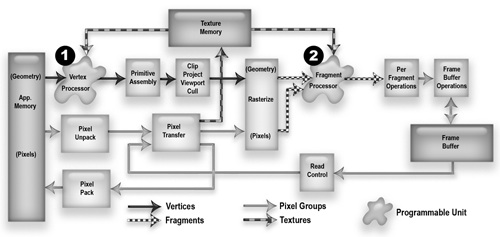
\includegraphics[width=4in]{graphicsProcessorModel.jpg} 
   \caption{Logical diagram of OpenGL's Programable Processor courtesy of \cite{glslRost}.}
   \label{fig-programable-processor}
\end{figure}

One language that has emerged from glslang is called the Core Image Kernel Language \cite{apple-core-image}, \cite{ciklReference}.  CIKL is a subset of glslang that limits the definition of loops or conditional statements to those that can be determined at compile time.  This implies that branches are restricted in the compiler's intermediate language.  The reference makes no mention as to whether the back-end of the compiler is the same as glslang.  Since the front end compiles to an intermediate language that is a proper subset of the glslang intermediate language, the assumption that the back-ends are the same is a fair assumption.  Any program that follows this model is a pseudo zero-branch program.


A Core Image Unit Kernel is a pseudo zero-branch program which is defined in terms of each pixel in a defined region of interest (ROI).
A ROI is specific set of points (pixels) by which a kernel may operate on.  There may be multiple ROI, one for the destination image and one for each input image.   A CI Filter object provides a region of interest which may be overwritten to specify a ROI for each input image.  The ROI for the destination is specified on the call of the CI Kernel itself, which by convention of the construction of CI Filters is invoked inside of the output image method.


CIKL includes a compare instruction.  This compare instruction is not a branch instruction.  It simply provides one of the two provided values based on the less than operation included in the instruction. The compare operation compares, in the scalar case,  an input denoted $x$, and returns either the second input, $y$, if $x < 0$ and the third input, $z$, otherwise.  The vector version performs the selection on each element of the vectors $\vec{x}, \vec{y}$, and $\vec{z}$ respectively.


Each kernel function is defined in terms of each of the input vectors, scalars, image samplers, and  destination pixel, whose coordinate is given by the destination coordinate function.  
Any of point in an input image sampler may be accessed through the ``sample'' function.  These points are defined within the ROI for the image samplers and Definition of Domain (DOD), a special form of ROI specific for the destination image.  It is typical to define a kernel which isolates the specific point in the input samplers and performs some fundamental mathematical operation on these points.  Mathematical operations include scalar and dot vector versions of  trigonometric operations (cosine and sine), addition  subtract, multiply, division, and modulus.



\subsection{Core Image Kernel Model}
%If no branches in the main process, then where?  -- Hybrid Approach 
There is a hybrid approach between CPU and GPU models that can generate modules which are pseudo-zero-branch.  
%Turing completeness requires the ability control of the execution pointer.  
A pseudo-zero-branch program is not zero-branch.  The programs assembled to form this hybrid approach are written in CIKL, and therefore have no branch in their definition.   Even if the functions composing these program have no branch, a pseudo-zero-branch program still includes the function call to calling these CIKL program.  
The CPU furnishes the branches necessary to combine each module into a structure satisfying the desired calculation.  The result of this hybrid approach is that the CPU builds zero-branch programs to be executed on the GPU.   Optimization of this hybrid approach becomes a function of well chosen modules, the reuse of constructed modules, and a parallel construction of reused modules.


To compute problems that involve that require iteration, the CIKL is extended by a class CI Filter Generator.  It is a class meant to execute on a general purpose architecture, such as IBM's PowerPC or Intel's multiple core x86 processors.  The filter generator connects smaller filters together.  The filter generator aides the CIKL compiler in optimizing the filter code for the OpenGL Programable Processor.

The author of this paper introduces a mathematical model which is can be implemented in CIKL.  Any model that uses the CIKL is called a CI Kernel Model.  The specific mathematical model introduced in this paper is called Neighborhood Algebra.  Neighborhood algebra is an extension to classical linear algebra.  The paper illustrates the extension operations, and complement operations which obey the classical linear algebra constraints.  

Neighborhood algebra contends with one other caveat which the CIKM requires. 
No destination pixel can be reused as an input pixel for the kernel itself.  This would force an order dependency which is not supported in the CIKM.  In order to perform such operations, one kernel must supply its output image as an input image to another, as shown in sub-section \ref{cifiltergenerator}. Each of the points are determined in parallel via the vector pipelines, which are specified in the GLSL specification.  The kernel then becomes a pipelined structure, and provides the efficiency of the CIKM.

\subsection{Constructing Where Size and Position Matters}\label{cifiltergenerator}

%CI Filter Generators fundamental connection
As stated the results of a CI Kernel can be used as an input to another CI Kernel.  The CI Filter object encapsulates each respective CI Kernel.   In principal, any loop can be used to insert images, both original and outputs of CI Filters, into more CI Filters.   This process can  encapsulate and define complex filters using what is called a CI Filter Generator.  A CI Filter Generator provides a connect object method to connect one CI Filter, number or vector to another CI Filter, and form a structure of these connections.    The structure itself is capable of forming an archive which can be saved and passed on to other processes.      

%What they export
This structure can also be used to construct another CI Filter.   Such a CI Filter is the compilation of the CI Filter Generator's member filters.   The definition of the CI Filter is determined by the way each member filter is connected. % connection of filter in the CI Filter Generator defines the specifics of the constructed filter.  
The resulting filter is a stored object which the CIKL compiler constructs into a concise filter.   The resulting filter constructed by a CI Filter Generator can be used by another CI Filter Generator.  

%Where they define their meaning
Thus a CPU-bound loop can assemble any complex CI Filter through a CI Filter Generator instance from less complex filters.  It is typical to define the inner loop of a particular process as a CI Filter (constructed by a CI Filter Generator instance), then use a CPU bound loop to connect each inner loop filter to each other.  The just-in-time compiler determines the dependencies and how many pipelines are needed to perform the computation optimally.  

%How they export
There are special items in addition to the connecting filters that define a CI Filter Generator's output filter.  Each CI Filter Generator supplies a dictionary defining the name, description and other special attributes of the constructed filter.  Also, each CI Filter Generator supplies export keys to define the input ports and output image of the resulting CI Filter.

In order to provide a computation model satisfactory to the constraints of the CIKL model, this paper introduces an extension to classic linear algebra called Neighborhood Algebra.  Neighborhood Algebra bends the definition of a column vector to produce a matrix structure more applicable in the GPU bound world.  

\section{Neighborhood Algebra}\label{neighborhood-algebra}
As mentioned in the mathematical background section, there is another way to compute the mixing matrix for determining principal components, namely Gram-Schmidt Orthogonalization.  In CPU form, the iterative nature of EVD and SVD.


\subsection{Neighborhood Orientation to Linear Algebra}
The mathematics associated with this neighborhood orientation is called, in this report, Neighborhood Algebra (NA.)   A neighborhood is treated as analogous to a column vector in standard linear algebra.  A neighborhood is a $k \times k$ image extracted from the image itself.  Neighborhoods are arranged horizontally forming a $k \times kN$ image where $N$ is the quantity of neighborhoods, which is shown in Figure \ref{neighborhoodArrangement}.  %This choice is made based on neighborhood nature of filtering, and inherent properties of ROI structures. 
This horizontal image structure of $k \times kN$ pixels is called a mixing image (succinctly, a mixer.)
%A third kernel filter produced for this report, which crops and translocates specific neighborhoods, is ROI extract, which copies out a region of interest as the name implies.  
This neighborhood orientation has advantages in image processing operations.  Dot multiply and addition are simpler operations than full matrix multiply, which is an example of the motivation for this neighborhood orientation.   

\begin{figure}[htbp] %  figure placement: here, top, bottom, or page
   \centering
   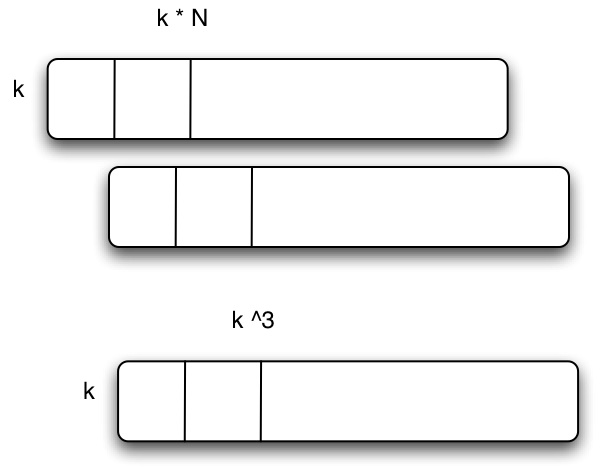
\includegraphics[width=5in]{../../assignment1/combinedReport/neighborhoodArrangement.jpg} 
   \caption{This diagram shows the arrangement of neighborhoods in a neighborhood mixing image. }
   \label{neighborhoodArrangement}
\end{figure}



\subsubsection{Gram Schmidt Orthogonalization motivated by Neighborhood Algebra (NA)}

GSO is an example of a linear algebra operation that benefits from neighbor orientation, and becomes a means of achieving parallelism in the construction of the CIKM generated filter for GSO.
Inner products computed in these cases reduces to one dot multiply between two neighborhoods, followed by $k$ sums.   Norms of the neighbors is one dot multiply, and $k$ sums of the elements inside each neighborhood. The scale and subtract is even more straight forward.  The scaling operation dot divides the inner product image by the norm image.  The resulting image is used to scale each neighborhood via the neighborhood scale kernel filter.  The final subtract filter subtracts a selected neighborhood from the working neighborhood and repeats this process for each neighborhood in the mixing image.  The caveat of the scale and subtract filter is that the neighborhoods in the scaled mixing image from the working neighborhood to the right are zeroed.  This allows for the scale and subtract to be general for each inner loop.



\subsection{Operations special to Neighborhood Algebra}
This section defines the kernel operators, mentioned earlier, composing the neighborhood oriented algebra operations necessary for GSO.  This section also connects these operations into compound operators, which have general use in neighborhood oriented algebra.  
The first group of kernel operators are ROI extraction, outer product, neighborhood scale and inverse scale.
%There are essentially two types of operations neighborhood algebra.  The first are kernel operators, which take some images and floating point arguments and return images.  The second are compound operators.  Compound operators consist of kernel operators combined together, often constructed by loops.  %Of the kernel operators, some have simple coordinate relations and others are defined in terms of ROI.   
%There is a third category required for GSO dependent on the comparison function.  

Neighborhood extraction, equation \ref{roiExtraction}, takes a specific neighborhood from a mixer and returns it as one neighborhood image.  Outer product, in neighborhood algebra and shown in equation \ref{outerProduct}, is a one kernel operator (for one neighborhood.)  Of course, the presence of multiple outer products is a compound operation using NA specific operations such as neighborhood extraction, and operations common to NA and classic linear algebra (CLA) namely dot multiply and subtraction.  


\begin{eqnarray}
		C = O_I(A,m,n) \\
		c_{(r,c)} = a_{(r+km, c+kn)} \label{roiExtraction}\\
		C = f_{O_1}(A,B) \\
		c_{r, c}  = a_{(\frac{r}{k}, c \bmod k)}  b_{(\frac{r}{k}, c \bmod k)} \label{outerProduct}
\end{eqnarray}
Neighborhood scaling is for scaling individual neighborhoods within a mixer.  Both a multiply and divide are provided, called scaling and inverse scaling.  The size of image $P$ in both equations \ref{nScaling}, and \ref{iNScaling} must be $1 \times N$, and $A$ must be $k \times kN$ where $k$ is the neighborhood size, and $N$ is the number of neighborhoods.  

\begin{eqnarray}
		C = f_N(\mathbf{A},M) = A \cdot_S P \\
		c_{r,c} = {a_{r, c}} {p_{(r \bmod {k}, c \bmod {k})}} \label{nScaling}\\
		C = f_N^{-1}(\mathbf{A},\mathbf{P}) = f_N (\mathbf{A}, 1\cdot/\mathbf{P}) = A \cdot_S^{-1} P \\
		c_{r,c} = \frac{a_{r, c}} {p_{(r \bmod k, c \bmod k)}} \label{iNScaling}
\end{eqnarray}

Sample selectors, conversions between CLA matrices and NA mixers, and the mix-match expansion have slightly more detailed coordinate transformations.  There are many transformations that even more detail, yet these kernel operations provide a crucial link needed to build the mixer for GSO.  The sample selection shown in equations \ref{sampleSelectorBeginning} through \ref{sampleSelectorEnding} take an image $A$, extracts $mn$ neighborhoods into a mixer.  The mixer, $\mathbf{C}$, is of size $k \times kmn$.  

\begin{eqnarray}
	\vec{v}_d = (r, c) ^T \label{sampleSelectorBeginning} \\
	t_s = \frac{c}{k} \\
	t_p = t_s / t_n \\
	p_s = {MN} t_p  \\
	\vec{v}_o = ( \frac{p_s}{k} , p_s \bmod k) \\
	\vec{v}_s = \vec{v}_o + \vec{v}_d \\
	C_{v_d} = A_{\vec{v}_s} \label{sampleSelectorEnding}
\end{eqnarray}

The mix-match expansion takes in a mixer, an image (size $M \times N$,) and floating point number indicating the iteration of the mixing step to define an image of size $Mk \times Nk$.  The purpose of this expansion is to provide the image equivalent to the neighborhoods being represented in CLA matrices in column (row) form.   From there a selection can be made based on estimating mixers for segmentation purposes.  Likewise, a de-mixing can be made as well.  This method can provide a powerful filtering mechanism for noise reduction.  The coordinate conversion of mix-match expansion shown in equations \ref{mixMatchExpansion} through \ref{mixMatchExpansionEnd} accomplishes this desired transformation.

\begin{eqnarray}
\vec{v}_d = (r,c)^T \label{mixMatchExpansion}\\
\vec{n}_d = (r \bmod k, c \bmod k) \\
\vec{m}_o = (0.0, k \tau) \\
\vec{m} = \vec{m}_o + \vec{n}_d \\
\vec{s} = (\frac{r}{k} , \frac{c}{k}) \\
k_2 = \lfloor \frac{k}{2} \\
\vec{k}_o = \vec{n}_d  - (k_2, k_2)^T \\
\vec{\alpha} = \vec{s}  + \vec{k}_o \\
c_{\vec{v}_d} = a_{\vec{\alpha}} b _{\vec{m}} \label{mixMatchExpansionEnd}
\end{eqnarray}

One transformation that is useful in other pattern classification techniques is the CLA to NA mixer kernel.  This transformation, and its inverse provide a vital link to methods determining estimators of many different kinds.  Equations \ref{beginCLAtoNA} through \ref{endCLAtoNA}  show the fundamental relationship between CLA matrices and NA mixers.  
\begin{eqnarray}
	\vec{v}_d = (r, c)^T \label{beginCLAtoNA}
	\vec{v}_o = (0.0, k  [\frac{c}{k}] )^T \\
	\vec{v}_i = \vec{v}_o - \vec{v}_i \\
	v_l = (v_i.x k + v_i.j , [\frac{c}{k}] )  \label{endCLAtoNA}
\end{eqnarray}

The general purpose compound operations are ones that the CLA world has used for decades and centuries.  The only difference in this case is the neighborhood orientation.  Neighborhood inner product for one neighborhood, shown in equation \ref{innerProductNA}, still $T$ dot multiplies where $T$ is the number of neighborhoods.  Similarly, norms, shown equation \ref{normsNA}, take the same number summations of kernel operations.   Neighborhood sum and mean (shown in equations \ref{sumsNA} and \ref{meanNA}, respectively) also require $T$ sums which is implicit with their names.
\begin{eqnarray}
	I_p(A, S, T) = \sum_{t \in T} (O_I(A,0,t) O(A,0,S)) \label{innerProductNA} \\
	N(A, T) = \sum_{t \in T} (O_I(A,0,t) O(A,0,t)) \label{normsNA} \\
	C = \sum _N O_I (A, 0, N ) \label{sumsNA} \\
	C = \frac{1}{N} \sum _N O_I (A, 0, N ) \label{meanNA}
\end{eqnarray}



\subsection{Extensions on Gram Schmidt Orthogonalization into Neighborhood Algebra }
One necessary abuse of Neighborhood algebra to compute GSO is the last components of the inner loop GSO compound operation.  GSO Subtract, $G_s (\mathbf{I}, \mathbf{S}, I_c, S_c)$, is the final subtract of the mixer for the GSO Inner Loop.  It is meant to subtract the neighborhood sum of $c_i w_i$ just like the CLA version shown in equation \ref{GSTheorem}.  The compound operation at the final leg of that makes the inner loop of GSO is shown in equation \ref{gsoDivision} through \ref{gsoSubtract}.  Because, $Q'$ is determined by a loop on $G(\mathbf{I}, \mathbf{S}, I_c, S_c)$, $Q'$ is also a compound operation which is called GSO estimate, $G_E(I_p(\mathbf{A},s,t), N(\mathbf{A},t))$.  

\begin{eqnarray}
D(I_p(\mathbf{Q},S,T), N(\mathbf{A},t) ) = \frac{I_p(Q,s,t)} {N(\mathbf{Q},t)} \label{gsoDivision}\\
Z(I, y)  = 
\left(
\begin{array}{llll}
 I(x,0) & ...  &  I(x,y) & 0 \\
 ... &  ... &   ... &  0\\
I(x,0)  &...   &   I(x,y) & 0
\end{array}
\right) \\
\mathbf{S} = \mathbf{A} \cdot_S Z(D(I_p(\mathbf{Q},s,t), N(\mathbf{Q},t) ) , y)  \\
Q' = \sum_{r=0}^{r<t} -(G_s (\mathbf{Q}, \mathbf{S}), r, t )) \label{gsoSubtract}
\end{eqnarray}

The outer loop of GSO connects the inner loops of GSO by counting out the neighborhoods, and consists of feedback from each iteration.  

Another extension necessary to execute GSO in NA is the concept of a scatter matrix.  In this case, the zero-mean is not considered, but the NA equivalent of $\mathbf{A}\mathbf{A}^T$ is.   The input for this scatter matrix requires $\mathbf{I_N}$ to be $k \times kn$ where $n$ is the number of samples in the neighborhood sample mixer. The result of neighborhood scatter, $f_S (\mathbf{I_N})$, is $\mathbf{I_S}$, which is $k \times k^3$.  It is this $\mathbf{I_S}$ which GSO is applied to, and generates the PCA estimate.  Algorithm \ref{alg:neighborhood-scatter} shows the inner loop neighborhood scatter operation.  This operation for a given $k_n$ is the loop count.  The loop length is of size $n$, which accounts for the NA equivalent of matrix multiply.  

\begin{algorithm}
\caption{Neighborhood Scatter}
\label{alg:neighborhood-scatter}
\begin{algorithmic}
	\REQUIRE $\mathbf{I_N}$ of size $k \times kn$
	\REQUIRE $k_n$, the 
	\REQUIRE $\vec{v_c}$ the destination coordinate in $I_S$
	\STATE $j \leftarrow floor(\vec{v_c}.y / k)$
	\STATE  $d \leftarrow \vec{v_c}.y - j k$
	\STATE $i \leftarrow \vec{v_c}.x * k + d $
	\STATE $\vec{v_l} \leftarrow$ vec2 ($i,j$)
	\STATE $\vec{v_{al}} \leftarrow$ vec2 ($\vec{v_l}.x, k_n$)
	\STATE $\vec{v_{atl}} \leftarrow$ vec2 ($k_n, \vec{v_l}.y$)
	\STATE $\vec{a} \leftarrow$ xformCLAtoNA ($\vec{v_{al}} , k$)
	\STATE $\vec{b} \leftarrow$ xformCLAtoNA ($\vec{v_{atl}} , k$)
	\STATE $\vec{\alpha} \leftarrow$ sample (src, $\vec{a}$)
	\STATE $\vec{\beta} \leftarrow$ sample (src, $\vec{b}$)
%	\RETURN 
	\ENSURE $f_S(\mathbf{I_N}) = \mathbf{I_S}$ s.t. $\mathbf{I_S}_{\vec{v_c}} = \vec{\alpha} \cdot \vec{\beta}$
\end{algorithmic}
\end{algorithm}

So for an PCA estimate of the neighborhoods of a given image, $f_{\textrm{PCA}}$, the estimate must acquire the samples, apply neighborhood scatter, and apply GSO to that scatter as stated mathematically in equation \ref{pca-estimate-NA}.
\begin{equation}
f_{\textrm{GSO}} (f_S (f_{\textrm{ESM}}(\mathbf{I}) )) \label{pca-estimate-NA}
\end{equation}
This estimate is the mixer required for the mix-match expansion and the inverse of equation \ref{pca-estimate-NA} is needed for the neighborhood reduction, along with a selection of $p$ from the $k \times k$ PCA choices.  

\section{GPU-bound products using Quartz Composer}
%What is Quartz Composer?
Quartz Composer (QC) is a rapid development environment tool that allows a developer or user to use concise units, called patches, to construct powerful graphics oriented effects.  QC provides the user with a set of filters, generators, input patches, composite patches and plug-ins to construct effects while contributing very little program code.  The plug-in patches and SDK provides developers the ability to test their own code, which they provide in an intuitive manner.  QC was shown in the CPU-bound implementations of PCA and ICA in a report written prior to this paper\cite{beatty-report-mitra}.    

The CPU bound QC plug-ins used dictionaries to pass data from patch to the next, as the primary matrix data type is only indirectly supported.  Also, optimizations on handlers were required to ensure that no plug-in took to long to perform a computation.  This limitation causes EVD to be limited to a size of 49 by 49 when using LAPACK's implementation,  otherwise QC would become die due to a time limit safeguard.   This limit causes the neighborhoods to be limited to 7 by 7, and justifies the investigation into a GPU bound version.  

There are three issues to building prototypes in QC using CLA or NA as a mathematical model, which have to do with connecting filters to form a super filter.  One is the loop control.  The other is the conditional filter.   Third issue applies to control over the ROI/ DOD for each filter, which are simplified in the Objective-C implemented CI-Filters and not as well documented in the QC CI Kernel Patch. 


The iterative feedback loop control is a QC Plug-in essential to the construction of super filters using the QC tool.  The feedback control loop itself has three inputs.  The two images, initial and feedback, supply the control with a selection to start and finish the loop.  The loop limit controls how many loops may be executed.  This works well with the neighborhood algebra model as it is typically the height of the image being computed.  The outputs of the feedback control loop patch are the result image and the loop index.  The result image is fed into the compositions components, which define the unit's inner loop.  The loop index, as the name implies, is the index for the inner loop's components to work on.   This is a consequence of the neighborhood algebra model and does have a design pattern to it. 

The iterative feedback loop controller inherently must store the feedback image in the event the count limit is reached.  In that event, the stored image and not the incoming feedback image is supplied as output.  This causes the connected patches to see no change, and therefore not execute.  Without this safeguard, the loop controller would supply its last feedback image as the input image to the connected patches.  Since this would be a new image, the connected filter would execute.  The result would eventually come back to the feedback loop controller, and the cycle would be continue indefinitely.


At one time there was a consideration for implementing the iterative feedback loop control as a CI Filter.   This thought led to the construction of the conditional filter.  It is a rather simple Objective-C CPU bound filter.  It takes three inputs, two images to choose from and the truth value (a number).   The output image of the conditional filter one of the two input images selected on the basis of the truth value.  The caveat is the termination safeguard.

%What are Quartz Composer plug-ins 
%In this sub-section, QC plug-ins are further elaborated to aid in understanding QC's prototype assisting power.  In both cases, developing a CPU-bound filter and a CIKM filter, the dictionary type (NS-Dictionary ) is key to moving these data-types from patch to patch.  This particular dictionary type can store any object type, and it is useful to pair that object with a standardized key.  In the case of CIKM types, the key used is ``CIFilter,'' which is the precise data type used and produced.  

%Also in this sub-section an incremental approach is made by reducing the QC Plug-in to a loop controller with feedback.  This concept allows kernel level CI Filters to be connected directly in QC without using a dictionary as a wrapper.  The advantage is that the prototype is reduced in complexity.  The disadvantage is rooted in the selection and copy of either the feedback or initial images.  
In both the Objective-C implemented filters and the QC prototypes, control of the ROI and DOD are critical to NA.   Control of the ROI allows shifting of the working window, scaling, blending and pixellating operations.  Control of the DOD ensures that operations that yield the new dimensional sizes, which forces obediance to the NA and CLA.   The only difference between the Objective-C and QC prototypes is that the ROI and DOD are set via  JavaScript in the QC prototype, as opposed to Objective-C for the CI image unit.   
	
	There are benefits from the control loop model. First, the prototype reduces all CI Filters to kernel level.  Each patch can be reduced to unit purpose. Each unit purpose patch has a direct resemblance to its neighborhood algebra model. Lastly, the native CI patch can be used to reduce the CI Filter plug-in's, reducing the number of filters necessary to distribute.  

	The inner loop of GSO in this feedback control loop model obeys the neighborhood algebra model.  The inner product and norms results are fed into the subtraction composition.  The input to both inner product and norms compositions are either the initial image or feedback from the subtract composition.  The loop and determination of the input to the inner loop is controlled by the feedback and control plug-in.  

	The inner product composition also obeys the neighborhood algebra model and has a feedback control patch.  The same can be said about norms and the subtraction composition.  As the neighborhood model specifies the number of neighborhoods is the ratio of width to height, the dimensions' patch in combination with a math patch determines these values.   These patches can be observed in Figure \ref{controlLoopGSO}.   

	\begin{figure}[htbp] %  figure placement: here, top, bottom, or page
	   \centering
	   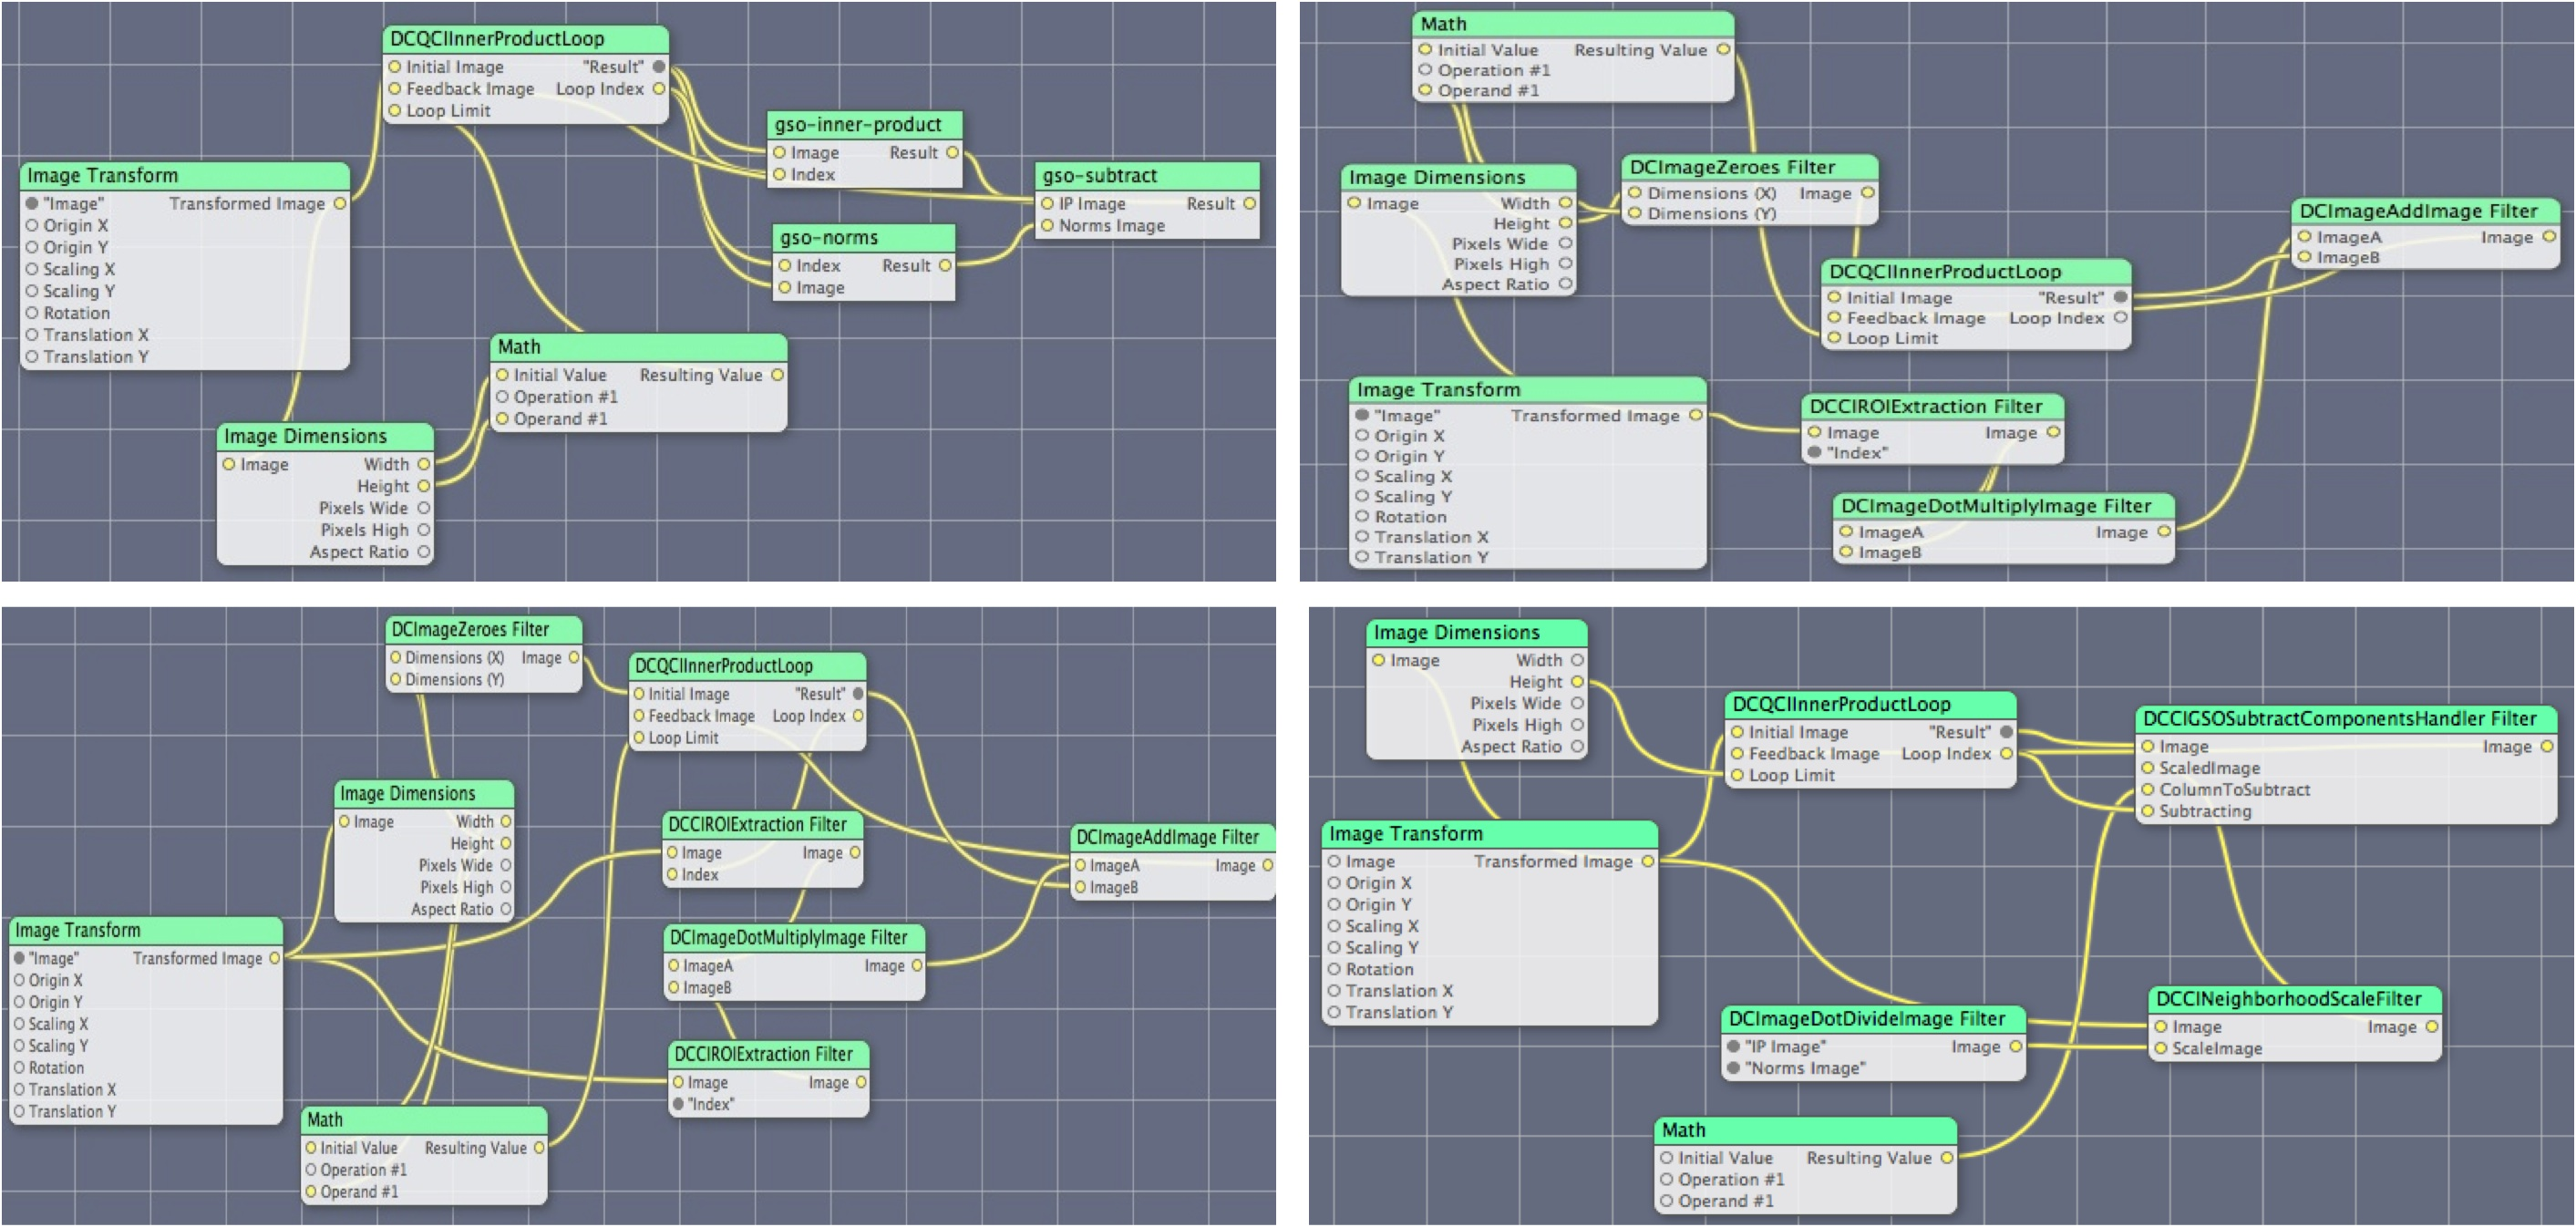
\includegraphics[width=6in]{../../assignment1/combinedReport/controlLoopGSO.jpg} 
	   \caption{This diagram shows the collection of QC patches computing GSO using a feedback control patch.  Called DCQCIInnerProductLoop in these diagrams, the control patch provides a mechanism for feedback to build a solution for the PCA mixing matrix.  This approach empowers QC to provide prototyping tool for GPU bound solutions.}
	   \label{controlLoopGSO}
	\end{figure}



\section{Accelerate Construction of CIKM using NSOperation}\label{nsoperation-for-cifilter-generator}
There is a method for altering a handler, originally made for a Quartz Composer plug-in, to inherit multi-threaded properties by making it a NS-Operation subclass. % to being a subclass of NSOperation, which inherits multi-threaded properties.  
There are three key differences which do not effect the logic, but supply parallelism to the computation.  First the algorithm specified in the ``determine'' method becomes the ``main'' method.  Second, the properties passed by other handlers must be accessed from the other handlers and the other handlers become dependent properties of the operating handler.  These handlers must be specified as dependencies.  Third, the handlers become operations themselves, and those operations must be loaded into an NS-Operation Queue while the queue is suspended.   Once loaded, the queue may be reactivated, which causes the handlers to be determined in parallel fashion.  
%One key to that transformation is making the determine method the main method, and altering the input filters to being handlers that generated them.   The other part is to stop the NS-Operation queue while loading operation objects into the queue.  

% Basic Loop concept 

% Proper use of feedback 

% Issue of in and out protocols for QC-Plugin images.  


% Neighborhood algebra


% Norms 
% Dot divide 
% Neighbor scale
% GSO Subtract

% Neighbor expansion
Figure  \ref{qc-gso-fundamental-core} shows the Quartz Composer patch connection method of combining these filter generating handlers.  The filters can be converted to NS-Operation subclasses with relative ease.  This conversion allows for a NS-Operation Queue to determine the final filter.  There are two possibilities of deployment via this queue.  The queue can be inserted into a CI-Filter plug-in as a CPU component of the filter.    The advantage of the pseudo filter is that it is usable in Quartz Composer and is treated as a kernel filter. This is sort of  pseudo filter can have one disadvantage.  The disadvantage is the filter may not be reused without being regenerated.  Also, the filter does have to wait for the queue to finish computations.  On single CPU systems, that queue could take more time than the security model allows.   


% Show the handler construction

% identify the problem for QC

% QC: Use plug-in patches to form the loop control, and use feedback to perpetuate the inner loop. 

%  Show the non-threaded gerneration.

%  Show the NS-Operation version


\bibliography{../../patternNotes.bib}
\bibliographystyle{abbrv}
\end{document}